\chapter{Codificação de Fonte}

A codificação de fonte sem perdas é o objetivo central quando
buscamos representar os símbolos de uma fonte estocástica de forma eficiente.
Ou seja, desejamos utilizar o menor número de bits possível para
codificar a informação produzida pela fonte, sem que haja perda de informação,
sendo assim possível reconstruir no receptor, exatamente a mesma mensagem
enviada pelo emissor.

O Teorema da Codificação de Shannon estabelece que, para uma fonte com entropia
$H(X)$, é possível codificar utilizando uma taxa $R > H(X)$ bits por símbolo,
desde que se empregue blocos suficientemente grandes. No entanto, a codificação
por blocos pode ser impraticável em aplicações reais devido à latência e à
complexidade computacional, o que motiva a busca por alternativas mais práticas
que ainda alcancem o limite teórico da entropia.

Neste capítulo, exploraremos duas abordagens principais: códigos de tamanho
variável, como a Codificação Huffman, que atribui palavras-código de
comprimento variável a símbolos individuais, e a codificação de fluxo
(\textit{stream coding}), que opera no fluxo de dados considerando o símbolo
atual e sua história, como na Codificação Aritmética e na Codificação
Lempel-Ziv --- esta última sendo universal, pois não requer conhecimento prévio
da distribuição $p(x)$. Assumiremos que a distribuição $p(x)$ da fonte é
conhecida ou que uma aproximação $q(x)$ está disponível, e investigaremos o
impacto de utilizar $q(x)$ quando a distribuição verdadeira é $p(x)$, sem
abordar diretamente o problema de estimação de $p(x)$. Buscaremos
analisar métodos práticos que se aproximem do limite de entropia.

Para abordar este assunto, devemos inicialmente fazer algumas definições.

Um código, no contexto de codificação de fonte, é uma função que mapeia os
símbolos de uma fonte em sequências de bits (palavras-código) de forma a
representá-los. Usualmente, o objetivo em se estabelecer um código é minimizar
o número de bits necessário para transmissão ou armazenamento da mensagem
produzida pela fonte. Um código pode ser de tamanho fixo ou variável, e, para
codificação sem perdas, devemos requerer que cada símbolo seja
univocamente recuperado a partir de sua palavra-código.

\begin{definition}[Codificação de Fonte]
Um código $C$ para a v.a. $X$ é um mapeamento de $\mathcal{X}$ em $\mathcal{D}^\ast$,
ou seja
\begin{equation}
  C: \mathcal{X} \rightarrow \mathcal{D}^\ast ,
\end{equation}
onde $\mathcal{D}^\ast$ é o conjunto
de sequências (\textit{strings}) finitas em um alfabeto $D$-ário. $C(x)$ é a palavra código
(\textit{codeword}) correspondente ao símbolo $x$, e $l(x)$ é o comprimento desta palavra.
\end{definition}
De forma geral, $\mathcal{D} = \{0,1, \ldots, D-1\}$, mas usualmente utilizamos $D=2$, ou seja,
codificação binária com alfabeto $\mathcal{D} = \{0,1\}$.
O conjunto $\mathcal{D}^\ast$ representa a extensão do alfabeto $\mathcal{D}$
(fecho de Kleene\footnote{
  O fecho de Kleene de um alfabeto $\mathcal{D}$, denotado $\mathcal{D}^\ast$,
  é um conceito da teoria de linguagens formais que inclui todas as sequências
  finitas que podem ser formadas concatenando zero ou mais símbolos de $\mathcal{D}$,
  incluindo a sequência vazia, frequentemente representada por $\epsilon$.

} do alfabeto), consistindo de todas as sequências finitas (de qualquer tamanho,
incluindo a sequência vazia) formadas por símbolos de $\mathcal{D}$, excluindo
sequências infinitas, que seriam denotadas por $\mathcal{D}^\infty$.

\begin{example}
Seja $\mathcal{X} = \{\text{azul}, \text{vermelho}\}$. O código pode ser $C(\text{vermelho})=00$ e
$C(\text{azul})=11$, o que seria um código binário para $\mathcal{D} = \{0,1\}$.
Teríamos então $\mathcal{D}^\ast = \{ 00 , 11 \}$. Uma sequência produzida pela fonte da forma
$(\text{azul},\text{azul},\text{vermelho})$ seria codificada como $(11,11,00)$, ou melhor, $111100$.
\end{example}

O comprimento esperado de um código é uma medida fundamental na codificação de
fonte, pois quantifica a eficiência média do código ao representar os símbolos
da fonte, permitindo comparar diferentes esquemas de codificação em termos de
uso de bits.

\begin{definition}[Comprimento Esperado]
O comprimento esperado $L(C)$ de um código $C$ para uma v.a. $X$ com distribuição $p(x)$ é dado por
\begin{equation}
  L(C) = \sum_x p(x) l(x) .
\end{equation}
\end{definition}


\begin{example}
  Seja $\mathcal{X} = \{1, 2, 3, 4\}$ e $\mathcal{D} = \{0, 1\}$. Podemos definir
  o código através da \Cref{tb:excode1}.
  \begin{table}[h]
    \centering
    \caption{Código binário de exemplo para quatro símbolos.}\label{tb:excode1}
    \begin{tabular}{c|c|c|c}
      x & p(x)  & c(x) & l(x) \\ \hline
      1 & $1/2$ & 0    & 1    \\
      2 & $1/4$ & 10   & 2    \\
      3 & $1/8$ & 110  & 3    \\
      4 & $1/8$ & 111  & 3    \\
    \end{tabular}
  \end{table}
  Neste caso, teremos $H(X) = 1.75$ e $L(C)=El(X)=1.75$, então este código é muito bom.
  A decodificação para este código é fácil, por exemplo, dada a sequência binária 010110111111110100,
  podemos prontamente identificar a sequência de símbolos que a produziu: 1,2,3,4,4,3,2,1.
  Seria como se tivéssemos uma pontuação separando os símbolos: 0,10,110,111,111,110,10,0.
  Dizemos que o código possui pontuação automática.
\end{example}

\begin{example}
Vamos considerar $\mathcal{X} = \{1,2,3\}$ e $\mathcal{D}=\{0,1\}$.
O código proposto é apresentado na \Cref{tb:excode2}.
\begin{table}[h]
  \centering
  \caption{Exemplo de código binário para um alfabeto com 3 símbolos.}\label{tb:excode2}
   \begin{tabular}{cccc}
   x      &  1    &   2   &   3   \\ \hline
   $p(x)$ & $1/3$ & $1/3$ & $1/3$ \\ \hline
   $C(X)$ & $0$   & $10$  & $11$
   \end{tabular}
\end{table}
Para o código proposto, teremos então $El(X)=1.66 > H$ bits, uma vez que $H = 1.58$ bits.
Note ainda como podemos facilmente decodificar uma sequência, como $10110010 = 2,3,1,1,2$.
\end{example}

A eficiência de um código é uma medida que compara o comprimento esperado $L$
do código com a entropia $H(X)$ da fonte. Ela serve como um indicativo do
quão próximo o código está do limite teórico de
compressão estabelecido pelo Teorema da Codificação de Shannon.

\begin{definition}[Eficiência de um código]
  A eficiência de um código é definida da seguinte forma
    \begin{equation}
      0 \leq \text{eficiência} \triangleq \frac{H_D(X)}{E l(X)} \leq 1 .
    \end{equation}
\end{definition}

\begin{example}
  Para $\mathcal{X} = \{1,2,3,4\}$ e $\mathcal{D}=\{0,1\}$ (código binário), considere os seguintes códigos
  dados na \Cref{tb:excode3}
  \begin{table}[h]
    \centering
    \caption{Comparativo de 4 códigos distintos para uma fonte com 4 símbolos e distribuição dada.}\label{tb:excode3}
    \begin{tabular}{c|c|c|c|c|c}
    $x$           & $p(x)$& $C_I$ & $C_{II}$ & $C_{III}$ & $C_{IV}$ \\ \hline
    1             & 0.5   &  0    &   0   &  0            &   0   \\
    2             & 0.25  &  0    &   1   & 10            &  01   \\
    3             & 0.125 &  1    &  00   & 110           & 011   \\
    4             & 0.125 & 10    &  11   & 111           & 0111  \\
    $H(X)$        & 1.75  &  -    &  -    &  -            &  -    \\
    $El(X)$       &  -    & 1.125 & 1.25  &  1.75         & 1.875 \\
    eficiência    &       & 1.555 & 1.4   & 1             & 0.933 
    \end{tabular}
  \end{table}
  Neste caso, obtemos valores impróprios para os códigos $C_I$ e $C_{II}$,
  indicando que não podem ser códigos sem perdas, já que violam do teorema de Shannon.
  O valor esperado do comprimento do código não pode ser menor que a entropia sem que o código incorra em erro.

  Note que o código $C_I$ não é unívoco. A sequência $00001$ pode ser decodificada como
  $1,2,1,2,3$ ou $2,1,2,1,3$ ou $1,1,1,1,3$.

  Considere $C_{II}$. O resultado da decodificação de $0011$ poderia ser $,1,1,2,2$ ou $3,4$ ou $3,2,2$ ou $1,1,4$.
  Novamente, não é possível decodificar sem que a probabilidade de erro seja nula (quando a sequência torna-se mais longa, a probabilidade de erro tende a $1$).

  O código $C_{III}$ é factível (já que $El \geq H$). O processo de decodificação é simples. Por exemplo: $111110100 = 111,110,10,0 = 4,3,2,1$.

  Utilizando o código $C_{IV}$ é possível decodificar a sequência $00000000111$ univocamente, porém os símbolos não são instantaneamente decodificados, é necessário analisar os bits à frente para conseguir decodificar.
\end{example}


\begin{definition}[Extensão de um código]
Um extensão $C^\ast$ de um código $C$ é um mapeamento de uma sequência finita
de símbolos em $\mathcal{X}$ em uma sequência finita de símbolos em $\mathcal{D}$ através da
concatenação dos códigos:
\begin{equation}
C^\ast (x_1,x_2,\ldots,x_n) = C(x_1) C(x_2) \ldots C(x_n) .
\end{equation}
\end{definition}

Um código não-singular é uma função de codificação que mapeia os símbolos de
uma fonte estocástica em palavras-código de forma que cada símbolo tenha uma
representação única, sendo essa uma condição necessária para a codificação sem
perdas, embora não garanta por si só a decodificação unívoca.

\begin{definition}[Código não-singular]
Um código é dito \textbf{não-singular} se todo elemento de $\mathcal{X}$
é mapeado em sequências (\textit{strings}) diferentes em $\mathcal{D}^\ast$. I.e.,
\begin{equation}
x_i \neq x_j \Rightarrow C(x_i) \neq C(x_j) .
\end{equation}
\end{definition}

Para garantir que cada sequência codificada possa ser recuperada de forma inequívoca
a partir de sua representação em bits, um código precisa ter decodificação unívoca,
ou seja, não pode haver ambiguidades na decodificação.

\begin{definition}[Código com decodificação unívoca]
Um código $C$ com extensão $C^\ast$ é decodificável univocamente se a sua extensão $C^\ast$ for não-singular.
\end{definition}

Em um código de prefixo nenhuma palavra-código é um prefixo de outra, garantindo que a decodificação possa ser realizada de
forma unívoca e sequencial sem a necessidade de olhar para além do próximo delimitador.

\begin{definition}[Código de prefixo]
Um código é chamado \emph{código de prefixo} ou \emph{código instantâneo} se nenhum palavra
é prefixo de qualquer outra palavra.
\end{definition}

Quando temos um código de prefixo, sabemos onde está o fim de uma palavra, pois ela não
é prefixo de nenhuma outra, ou seja, não existe nenhuma outra palavra que comece com a palavra
dada. Podemos dizer que um código de prefixo possui então a propriedade de auto-pontuação.

Dentre o conjunto dos códigos unívocos possíveis, queremos um código com
comprimento esperado mínimo possível. Analisando as classes de códigos,
intuitivamente pensamos que é mais provável encontrarmos um código com
comprimento esperado menor em uma classe maior (ou mais abrangente). 
A \Cref{fig:tiposcodigos} apresentado a estrutura hierárquica dos códigos
(todos os códigos $\supset$ não-singulares $\supset$ unicamente decodificáveis $\supset$ prefixo).

\begin{marginfigure}%
  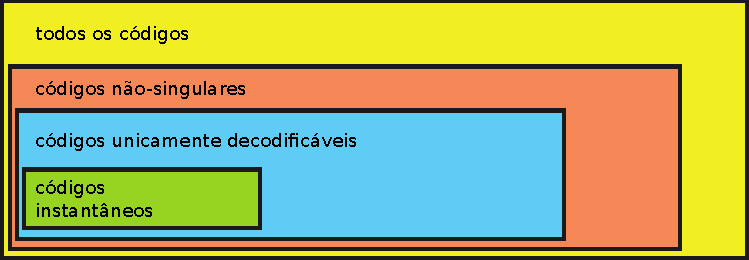
\includegraphics[width=\linewidth]{figures/tiposcodigos.pdf}
  \caption{Diagrama de representação dos conjuntos de códigos, evidenciando a estrutura hierárquica existente.}\label{fig:tiposcodigos}
\end{marginfigure}




\section{Desigualdade de Kraft}

A Desigualdade de Kraft estabelece uma condição necessária e suficiente para a
existência de códigos de prefixo com comprimentos de palavras-código
especificados. A demonstração, que será vista, ainda fornecerá um método para
construir um código de prefixo.

\begin{theorem}[Desigualdade de Kraft]\label{thm:deskraft}
Para qualquer código instantâneo (código de prefixo) sobre um alfabeto de tamanho $D$, o comprimento
das palavras $l_1, l_2, \ldots, l_m$ deve satisfazer
   \begin{equation}\label{eq:desigualdadekraft}
      \sum_i D^{-l_i} \leq 1 .
   \end{equation}
Por um outro lado, dado um conjunto de comprimentos de código satisfazendo a desigualdade acima,
então existe um código de prefixo com estes comprimentos.
\end{theorem}

Note que foi dito que existe um código de prefixo com aqueles comprimentos, não
significa que todos códigos cujos comprimentos satisfazem a desigualdade são
códigos de prefixo. Se existe um código não-instantâneo com comprimentos $l_i$
satisfazendo a desigualdade de Kraft, então podemos encontrar um outro código,
que terá a propriedade de prefixo, e que possuirá os mesmos comprimentos $l_i$,
consequentemente não alterando o comprimento esperado. Logo, será sempre melhor
escolher um código de prefixo.


\begin{proof}[Demonstração (Desigualdade de Kraft)]
Vamos representar o conjunto de códigos em uma árvore $D$-ária (não necessariamente balanceada),
conforme a \Cref{fig:Dtree}.

\begin{marginfigure}
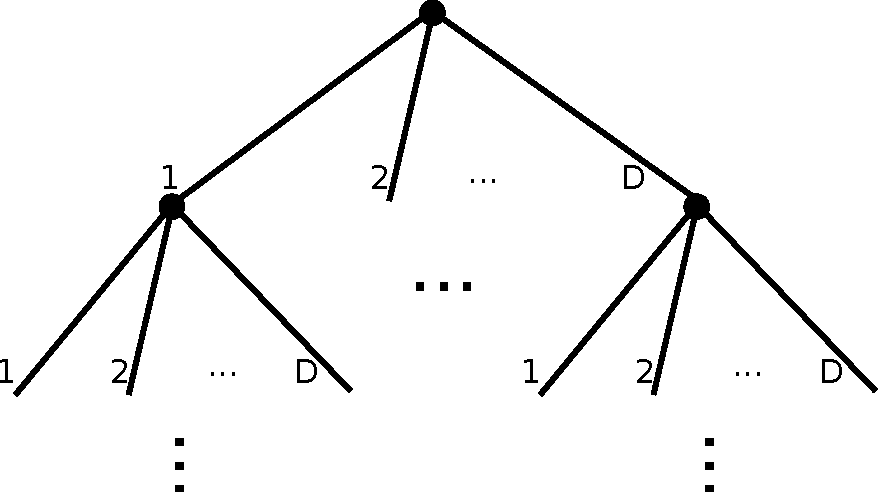
\includegraphics[width=\textwidth]{figures/Dtree.pdf}
\caption{Árvore $D$-ária.}\label{fig:Dtree}
\end{marginfigure}

As palavras correspondem à folhas na árvore. O caminho da raiz até a folha determina a palavra código.
A condição de prefixo implica que não existe uma palavra a não ser nas folhas
(nenhum descendente de uma palavra código será também uma palavra código).
$l_{\text{max}} = \max_i (l_i)$ é o comprimento da palavra mais longa.
Podemos expandir toda a árvore até o comprimento $l_{\text{max}}$.
Os nós no nível de $l_{\text{max}}$ são: palavras de código; descendentes de palavras de código; ou
apenas nós sem palavra código associada a ele ou seus antecessores.
Considere uma palavras $i$ no nível $l_i$ da árvore (então esta palavra possui comprimento $l_i$).
Existem então $D^{l_{\text{max}} - l_i}$ descendentes de $i$, na árvore, no nível $l_{\text{max}}$.
Com a condição de prefixo, podemos afirmar que os descendentes de código $i$ no nível $l_i$ são
disjuntos dos descendentes do código $j$ no nível $l_j$, quando $i \neq j$ (i.e., o conjunto de
descendentes para diferentes palavras é disjunto).
O número total de nós em um conjunto de todos descendentes é $\leq D^{l_{\text{max}}}$.
Utilizando o que vimos anteriormente, temos que a soma do número de descendentes de todos os códigos é menor ou
igual ao número de folhas na árvore cheia no nível $l_{\text{max}}$. Podemos então escrever
\begin{equation}
\sum_i D^{l_{\text{max}} - l_i} \leq D^{l_{\text{max}}} \quad \Rightarrow \quad \sum_i D^{-l_i} \leq 1 .
\end{equation}

Por outro lado, dados os comprimentos $l_1, l_2, \ldots, l_m$, satisfazendo Kraft, iremos mostrar como
construir um código de prefixo utilizando estes comprimentos.
Considere uma árvore $D$-ária cheia de profundidade $l_{\text{max}}$ e $D^{l_{\text{max}}}$ nós terminais.
Observe que: no nível 0 existe uma fração $1$ de descendentes de cada nó neste nível;
no nível 1 existe uma fração $1/D$ de descendentes de cada nó neste nível;
no nível 2 existe uma fração $1/D^2$ de descendentes de cada nó neste nível; e assim por diante.
De forma geral, em cada nível $i \in [0, l_{\text{max}}]$ da árvore, existe uma fração de $D^{-i}$
nós terminais que são descendentes de uma ramificação de cada um dos $D^i$ nós no nível $i$.
Ordene então os comprimentos $(l_1, l_2, \ldots, l_m)$ de forma ascendente $(s_1, s_2, \ldots, s_m)$,
sendo $s_1 \leq s_2 \leq \ldots \leq s_m$. Observe que existem tantos comprimentos quanto existem palavras.
Para o comprimento $s_1$, escolha um nó no nível $s_1$ para indicar o código.
Para garantir a condição de prefixo, o nó escolhido deve se tornar um nó terminal, eliminando assim uma
fração $D^{-s_1}$ de nós terminais no nível $l_{\text{max}}$.
Em seguida, escolha um dos nós remanescentes no nível $s_2$ (neste momento, existem $(D^{s_1}-1)D^{s_2-s_1}$
possíveis escolhas), eliminando assim uma fração $D^{-s_2}$ de nós terminais no nível $l_{\text{max}}$.
A fração total de nós eliminados, até o momento, foi de $D^{-s_1} + D^{-s_2}$.
Continuando este processo, iremos eliminar uma fração $\sum_{i=1}^{m} D^{-s_i}$ de nós, e neste processo
estamos garantindo que estamos criando um código instantâneo (uma palavra de código não pode ser prefixo de outra).
Como por suposição temos $\sum_{i=1}^{m} D^{-s_i} \leq 1$, nunca iremos eliminar mais do que todas as palavras
de código, então este processo não irá exaurir as palavras de código.
Criamos assim um código de prefixo com os comprimentos desejados, satisfazendo Kraft.
\end{proof}

A desigualdade de Kraft é uma condição \emph{sine qua non} (necessária e
indispensável) para a existência de um código prefixo.  A condição dada na
\Cref{eq:desigualdadekraft} deve ser satisfeita para que um dado código com
comprimentos $l_1, l_2, \ldots, l_m$ seja um código de prefixo.  A demonstração
também nos mostra como construir um código de prefixo, dado um conjunto de
comprimentos $\{l_1, l_2, \ldots, l_m\}$ que satisfaça a
\Cref{eq:desigualdadekraft}.


\section{Em busca do código ótimo}

Desejamos um código que forneça decodificação instantânea e livre de
ambiguidade, além disso, queremos um código eficiênte, que tenha comprimento
esperado mínimo. Desta forma, estamos em busca de um código de prefixo ótimo.

O comprimento esperado é dado por
\begin{equation}
  L(C) = \sum_{i} p_i l_i ,
\end{equation}
onde os comprimentos $l_i$'s devem ser números inteiros.
Teremos então o seguinte problema de otimização com restrição:
\begin{equation}
  \min_{\{l_{1:m}\} \in \mathbb{Z}_{+}^m} L(C) = \sum_i p_i l_i ,
\end{equation}
sujeito a
\begin{equation}
  \sum_i D^{-l_i} \leq 1 .
\end{equation}

Este é um problema de programação em inteiros que é um problema cuja
sua complexidade computacional cresce exponencialmente com o tamanho da entrada.
Não seria assim possível resolvê-lo de forma eficiente.
Vamos relaxar a condição de que $l_i$ precisa ser inteiro e considerar o Lagrangiano
\begin{equation}
  J = \sum_i p_i l_i + \lambda \left( \sum_i D^{-l_i} - 1 \right)
\end{equation}
Para encontrar os pontos estacionários de $J$, considerado uma função dos $l_i$'s
e do multiplicador lagrangiano $\lambda$, devemos encontrar as condições para que
as derivadas se igualam a zero, ou seja, $\sfrac{\partial J}{\partial l_i} = 0$,
$i=1,\ldots,m$, e $\sfrac{\partial J}{\partial \lambda} = 0$. Teremos assim
\begin{equation}
  \frac{\partial J}{\partial l_i} = p_i - \lambda D^{-l_i} \ln D = 0 ,
\end{equation}
e assim
\begin{equation}\label{eq:codotDli}
  D^{-l_i} = \frac{p_i}{\lambda \ln D} .
\end{equation}
Teremos também
\begin{equation}
  \frac{\partial J}{\partial \lambda} = \sum_i D^{-l_i} - 1 = 0 ,
\end{equation}
que nos fornecerá
\begin{equation}\label{eq:codotlambda}
  \lambda = 1 / \ln D .
\end{equation}
Utilizando as \Cref{eq:codotDli,eq:codotlambda} obtemos $D^{-l_i} = p_i$,
e assim os comprimentos ótimos são dados por
\begin{equation}\label{eq:codotli}
  l^\ast_i = -\log_D p_i .
\end{equation}
Desta forma, o comprimento esperado do código ótimo será
\begin{equation}\label{eq:codotLC}
  L^\ast = \sum_i p_i l_i^\ast = - \sum_i p_i \log_D p_i = H_D (X) = H(X) / \log D .
\end{equation}

Assumindo que seja possível utilizar comprimentos fracionários, os omprimentos
ótimos para as palavras de um código são $l^\ast_i = - \log_D p_i$, isto
implica que os comprimentos ótimos são iguais à informação do evento (o menor
comprimento para codificação de um evento é inerentemente a informação sobre o
próprio evento --- princípio da Navalha de Occam\footnote{
A Navalha de Occam, princípio atribuído ao frade franciscano Guilherme de Ockham 
(século XIV), sugere que, entre explicações concorrentes, a mais simples --- 
aquela que requer menos suposições --- deve ser preferida, desde que explique os 
fatos adequadamente. 
}), e assim o comprimento
esperado do código será a entropia.

Apesar os comprimentos ótimos dados na \Cref{eq:codotli} não seja, a princípio,
inteiros, podemos utilizar a codificação em blocos e assim proximar do limite
ótimo mesmo quando os comprimentos dos códigos por símbolos são valores fracionários.

\begin{theorem}[Comprimento esperado mínimo]\label{thm:comprespmin}
Entropia é o comprimento esperado mínimo. O comprimento esperado $L$ de qualquer código
$D$-ário instantâneo (satisfaz Kraft por conseguinte) para uma v.a. $X$ é tal que
\begin{equation}
  L \geq H_D (X) ,
\end{equation}
com igualdade sse $D^{-l_i} = p_i$.
\end{theorem}
\begin{proof}
  \begin{subequations}
    \begin{align}
      L - H_D (X) &= \sum_i p_i l_i - \sum_i p_i \log_D 1/p_i \\
                &= - \sum_i p_i \log_D D^{-l_i} + \sum_i p_i \log_D p_i \\
                &= - \sum_i p_i \log_D D^{-l_i} + \underbrace{ \log_D \left( \sum_i D^{-l_i} \right) - \log_D \left( \sum_i D^{-l_i} \right)  }_{=0} + \sum_i p_i \log_D p_i \label{eq:demthm:comprespminA}\\
                &= \sum_i p_i \log_D \frac{p_i}{r_i} - \log_D \left( \sum_i D^{-l_i} \right) \\
                &= \underbrace{D(p \mid\mid r)}_{ \geq 0} + \underbrace{\log_D (1/c)}_{ \geq 0} \\
                &\geq& 0 \label{eq:demthm:comprespminB}
    \end{align}
  \end{subequations}
  onde utilizamos em \ref{eq:demthm:comprespminA}, para simplificar, a soma de três das quatro parcelas é dada na \Cref{eq:demthm:simplificar},
  e em \ref{eq:demthm:comprespminB} utilizamos que $c \leq 1$ pois a desigualdade de Kraft deve ser satisfeita,
  onde $c = \sum_i D^{-l_i}$.
  \begin{subequations}\label{eq:demthm:simplificar}
    \begin{align}
      - \sum_i p_i \log_D D^{-l_i} + \log_D \left( \sum_j D^{-l_j} \right) +  \sum_i p_i \log_D p_i &= \\
      - \sum_i p_i \log_D D^{-l_i} + \left( \underbrace{ \sum_i p_i }_{=1} \right) \log_D \left( \sum_i D^{-l_i} \right) + \sum_i p_i \log_D p_i & \\  
      - \sum_i p_i \log_D D^{-l_i} + \sum_i p_i \log_D \left( \sum_j D^{-l_j} \right) + \sum_i p_i \log_D p_i &= \\
      \sum_i p_i \log_D \frac{p_i \left( \sum_j D^{-l_j} \right)}{D^{-l_i}} &= \\
      \sum_i p_i \log_D \frac{p_i}{\frac{D^{-l_i}}{\left( \sum_j D^{-l_j} \right)}} &= \sum_i p_i \log_D \frac{p_i}{r_i} ,
    \end{align}
  \end{subequations}
  onde definimos
  \begin{equation}
    r_i = \frac{D^{-l_i}}{\sum_j D^{-l_j}} .
  \end{equation}
\end{proof}

Assumindo que Kraft seja satisfeito (existe um código de prefixo com tais comprimentos)
teremos comprimentos inteiros de forma que $E l \geq H$. Se ainda $l_i = -\log_D p_i$ é
inteiro, para todo $i$, então teremos a igualdade $E l = H$. 
Se $l_i \neq -\log_D p_i$, mas $l_i$ é inteiro, teremos estritamente $E l > H$.


\section{Código de Shannon}
O código de Shannon é um código subótimo que consiste em considerar
o comprimento como inteiro mais próximo do valor ótimo, ou seja,
\begin{equation}\label{eq:compricodshannon}
  l_i = \lceil \log_D 1/p_i \rceil .
\end{equation}
Os comprimentos definidos desta forma satisfazem Kraft, uma vez que
\begin{equation}
  \sum_i D^{-l_i} = \sum_i D ^{- \lceil \log_D 1/p_i \rceil} \leq \sum_i D^{-\log_D 1/p_i} = \sum_i p_i = 1 .
\end{equation} 
Pelo \Cref{thm:deskraft}, existe então um código de prefixo com os comprimentos dados em \ref{eq:compricodshannon}.

\begin{theorem}[Limites para o comprimento esperado do código de Shannon]
  Sejam $l_1, l_2, \ldots, l_m$ comprimentos inteiros do código de Shannon para uma fonte $p$ e um
  alfabeto $D$-ário. $L$ é o comprimento esperado. Então
  \begin{equation}
   H_D(X) \leq L \leq H_D(X) + 1 .
  \end{equation}
\end{theorem}
\begin{proof}
Para o código de Shannon, teremos os seguintes limites:
\begin{subequations}\label{eq:limitescodshannon}
  %\begin{align}
      \begin{alignat}{2}
	  \log_D \frac{1}{p_i} & \leq l_i && \leq \log_D \frac{1}{p_i} + 1 \\
	  E_p \left[ \log_D \frac{1}{p_i} \right]  & \leq E_p \left[ l_i \right] && \leq E_p \left[ \log_D \frac{1}{p_i} + 1 \right] \\
	  \sum_i p_i \log_D \frac{1}{p_i} & \leq L && \leq \sum_i p_i \left( \log_D \frac{1}{p_i} + 1 \right) \\
	  H_D(X) & \leq L && \leq H_D(X) + 1 .
      \end{alignat}
  %\end{align}
\end{subequations}
\end{proof}

Observe ainda que, $H \leq L^\ast \leq L$, onde $L^\ast$ é o comprimento ótimo para códigos de comprimento inteiro.
Desta forma, também teremos a seguinte relação para o comprimento esperado de código ótimo: $H_D(X) \leq L^\ast \leq H_D(X) + 1$.

Podemos melhorar a eficiência do código de Shannon codificando mais de um símbolo por vez (codificação em bloco).
Vamos chamar de $L_n$ o comprimento esperado por símbolo de uma sequência de $n$ símbolos $x_{1:n}$. Então,
\begin{equation}
  L_n = \frac{1}{n} \sum_{x_{1:n} \in \mathcal{X}^n} p(x_{1:n}) l(x_{1:n}) = \frac{1}{n} E l(x_{1:n}) .
\end{equation}
tilizando os comprimentos do código de Shannon, teremos
\begin{subequations}
  \begin{alignat}{2}
    \log 1/p_i & \leq l_i &&\leq \log 1/p_i + 1 \\
    \sum_i p_i \log 1/p_i & \leq \sum_i p_i l_i &&\leq \sum_i p_i \left( \log 1/p_i + 1 \right) \\ 
    H(X_1,\ldots,X_n) & \leq E l(X_{1:n}) &&\leq H(X_1,\ldots,X_n) + 1 \\
    H(X) &\leq L_n &&\leq H(X) + \frac{1}{n} ,
  \end{alignat}
  onde utilizamos que $X_i$ são i.i.d., então $H(X_1,\ldots,X_n) = nH(X_i)$.
\end{subequations}
Quando $n$ cresce, a penalidade por símbolo imposta ao código de Shannon diminui e
conseguiremos assim aproximar-nos do limite da Entropia (por símbolo), embora teremos que
adotar a estratégia de codificação em blocos.



A escolha feita na \Cref{eq:compricodshannon} para definir o comprimento das palavras
no código de Shannon, subentende o conhecimento da distribuição $p$. Entretanto,
em geral, a distribuição subjacente não é conhecida. Isso implica que existem erros nos cálculos.
Suponha então que o código de Shannon utiliza $l(x) = \lceil \log 1/q(x) \rceil$, mas a real
distribuição é $p(x) \neq q(x)$. Vamos recalcular o valor esperado do comprimento do código,
agora utilizando esta informação. Encontraremos novos limites para o comprimento esperado
do código de Shannon.

\begin{theorem}[Limites para o código de Shannon com a distribuição aproximada]
O comprimento esperado de um código sob a distribuição $p(x)$ com $l(x) = \lceil \log 1/q(x) \rceil$ satisfaz
\begin{equation}
  H(p) + D(p \mid \mid q) \leq E_p l(X) \leq H(p) + D(p \mid \mid q) + 1 .
\end{equation}
\end{theorem}
\begin{proof}
Vamos analisar primeiramente o limite superior.  
\begin{subequations}
  \begin{align}
    E l(X) &= \sum_x p(x) \lceil \log 1/q(x) \rceil \\
           &\leq \sum_x p(x) \left( \log \frac{1}{q(x)} + 1 \right) \\
           &= \sum_x p(x) \left( \log \frac{p(x)}{q(x)} \frac{1}{p(x)} + 1 \right) \\
           &= \sum_x p(x) \log \frac{p(x)}{q(x)} + \sum_x p(x) \log \frac{1}{p(x)} + 1 \\
           &= D(p \mid \mid q) + H(p) + 1 .
  \end{align}
\end{subequations}
E agora, para o limite inferior temos
\begin{subequations}
  \begin{align}
    E l(X) &= \sum_x p(x) \lceil \log 1/q(x) \rceil \\
           &\geq \sum_x p(x) \log 1/q(x) \\
           &= \sum_x p(x) \left( \log \frac{p(x)}{q(x)} \frac{1}{p(x)}\right) \\
           &= \sum_x p(x) \log \frac{p(x)}{q(x)} + \sum_x p(x) \log \frac{1}{p(x)} \\
           &= D(p \mid \mid q) + H(p) .
  \end{align}
\end{subequations}
\end{proof}
Comparando estes limites com aqueles dados na \Cref{eq:limitescodshannon}, verificamos que
$D(p \mid \mid q)$ é o custo adicional por símbolo causado por utilizar a distribuição errada.



Um aspecto importante na análise de códigos é entender como seus comprimentos
de palavras se comparam a outros códigos univocamente decodificáveis em termos
de eficiência. O teorema a seguir aborda essa questão, fornecendo uma cota
probabilística para a diferença entre os comprimentos de palavras do código de
Shannon e de um código concorrente. Essa cota, expressa em função de uma
constante $c$, destaca a robustez do código de Shannon, mostrando que a
probabilidade de seus comprimentos excederem significativamente os de outro
código decresce exponencialmente, um resultado que reforça sua relevância.

\begin{theorem}[Otimalidade Competitiva do Código de Shannon]\label{thm:otcompcodshannon}
Considere $l(x)$ como o comprimento da palavra associada ao símbolo $x$ no
código de Shannon e $l'(x)$ como o comprimento da palavra correspondente em
outro código univocamente decodificável, ambos definidos sobre uma variável
aleatória $X$ com distribuição $p$. Então, a probabilidade de que
$l(X)$ exceda $l'(X)$ por pelo menos uma constante $c$ é limitada por:

\begin{equation}
\Pr \left( l(X) \geq l'(X) + c \right) \leq \frac{1}{2^{c-1}} .
\end{equation}

Equivalentemente, em notação mais formal:
\begin{equation}
\Pr \left( \mathbf{1}_{\{ l(X) \geq l'(X) + c \}} = 1 \right) \leq \frac{1}{2^{c-1}},
\end{equation}
onde $\mathbf{1}_{\{ \cdot \}}$ é a função indicadora.
\end{theorem}

\begin{proof}
    \begin{subequations}
      \begin{align}
        \Pr \left( l(X) \geq l'(X) + c \right) &= \Pr \left( \lceil \log 1/p(X) \rceil \geq l'(X) + c \right) \\
                                               &\leq \Pr \left( \log 1/p(X) \geq l'(X) + c - 1  \right) \label{dem:otcompcodshannonA}\\
              &= \Pr \left( p(X) \leq 2^{-l'(X)-c+1} \right) \\
              &=  \sum_{x:p(x) \leq 2^{-l'(x)-c+1}} p(x) \\
              &\leq \sum_{x:p(x) \leq 2^{-l'(x)-c+1}}  2^{-l'(x)-c+1} \\
              &\leq \sum_{x} 2^{-l'(x)} 2^{-(c-1)} \leq 2^{-(c-1)} \label{dem:otcompcodshannonB},
      \end{align}
    \end{subequations}
    onde em \ref{dem:otcompcodshannonA} utilizamos que o código de Shannon utiliza $l(x) = \lceil \log 1/p(x) \rceil$, e,
    em \ref{dem:otcompcodshannonB}, utilizamos a desigualdade de Kraft: $\sum_{x} 2^{-l'(x)} \leq 1$.
\end{proof}

A probabilidade do código de Shannon ter comprimento esperado maior do que um outro
código unicamente decodificável é exponencialmente decrescente com $c > 1$.
Código de Shannon é ótimo para distribuições d-ádicas, já que neste caso teremos que $\log 1/p(x)$ será inteiro.


Em distribuições $d$-ádicas, é mais provável que os comprimentos das palavra de
um código de Shannon sejam menores do que maiores em comparação com um código
alternativo. Esse resultado evidencia uma vantagem probabilística do código de
Shannon, destacando sua eficiência relativa.

\begin{theorem}[Otimalidade Competitiva do Código de Shannon II]\label{thm:otcompcodshannon2}
Considere uma distribuição $d$-ádica $p$ sobre um conjunto de símbolos,
onde $p(x) = 1/d^k$ para algum inteiro $k$, e seja $l(x) = \log_d (1/p(x))$
o comprimento da palavra associada a $x$ no código de Shannon, enquanto $l'(x)$
é o comprimento da palavra correspondente em outro código prefixo, ambos
aplicados a uma variável aleatória $X$ com distribuição $p$. Então:
\begin{equation}
\Pr \left( l(X) < l'(X) \right) \geq \Pr \left( l(X) > l'(X) \right),
\end{equation}
com igualdade se, e somente se, $l'(x) = l(x)$ para todo $x$.
\end{theorem}

\begin{proof}
Seja
\begin{equation}
\sign(t) = \begin{cases}
        1 , \quad t > 0 \\
        0 , \quad t = 0 \\
        -1 , \quad t < 0
        \end{cases}
\end{equation}
É fácil verificar que $\sign(t) \leq 2^t -1$ para $t=0,\pm 1, \pm 2, \ldots$.
Para $t = 0$ teremos $0 = 2^0 - 1 = 0$;
para $t \geq 1$ teremos $1 \leq 2^t - 1$, uma vez que $2^t > 1$ para $t \geq 1$;
e para $t \leq 1$ teremos $-1 \leq 2^t - 1$, uma vez que $2^t < 1$ para $t \leq 1$.

Teremos então
\begin{subequations}
{
\allowdisplaybreaks
\begin{align}
\Pr \left( l'(X) < l(X) \right) - \Pr \left( l'(X) > l(X) \right) &= \sum_{x:l'(x) \leq l(x)} p(x) - \sum_{x:l'(x)>l(x)} p(x) \\
             &= \sum_x p(x) \sign\left( l(x)-l'(x) \right) \label{dem:otcompcodshannon2A}\\
             &= E \left[ \sign \left( l(X) - l'(X) \right) \right] \\
             &\leq \sum_x p(x) \left( 2^{l(x) - l'(x)} - 1\right) \\
             &= \sum_x 2^{-l(x)} \left( 2^{l(x)-l'(x)} - 1 \right) \label{dem:otcompcodshannon2B}\\
             &= \sum_x 2^{-l'(x)} - \sum_x 2^{-l(x)} \\
             &= \sum_x 2^{-l'(x)} - 1 \\
             &\leq 1 - 1 \label{dem:otcompcodshannon2C} \\
             &= 0
\end{align}
}
\end{subequations}
onde em \ref{dem:otcompcodshannon2A} utilizamos que $\{l'(x) \leq l(x)\} \cap \{l'(x)>l(x)\} = \emptyset$,
em \ref{dem:otcompcodshannon2B} utilizamos que $p(x)$ é d-ádica, $p(x)=2^{-l(x)}$, e em \ref{dem:otcompcodshannon2C} 
utilizamos que $l'(x)$ satisfaz Kraft.
Assim, mostramos que $\Pr \left( l'(X) < l(X) \right) \leq \Pr \left( l'(X) > l(X) \right)$, como desejado.
\end{proof}




\section{Desigualdade de Kraft revisitada}
Considerando como objetivo principal, encontrar um código unívoco (unicamente decodificável)
com comprimento esperado de palavra mínimo, ao observar as classes de códigos, conforme
apresentadas na \Cref{fig:tiposcodigos}, podemos imaginar que a classe mais ampla é a mais
provável de se encontrar tal código desejado. Potencialmente, dentre os códigos
unicamente decodificáveis (um conjunto maior), podemos encontrar um código com menor comprimento esperado.
Entretanto, o teorema a seguir mostra que a desigualdade de Kraft é também
condição \emph{sine qua non} para obtermos um código unicamente
decodificável. Desta forma, podemos concluir que um código prefixo é a melhor escolha.

Primeiramente, vamos apresentar o seguinte lemma.
\begin{lemma}[Expansão Multinomial]\label{lm:expmultin}
  Seja $\mathcal{X} = \{x_1, x_2, \ldots, x_m \}$, $\vert \mathcal{X} \vert = m$, temos
  \begin{equation}
    \left( \sum_{x \in \mathcal{X}} D^{-l(x)} \right)^k = \sum_{x_{1:k} \in \mathcal{X}^k} D^{-l(x_1)} D^{-l(x_2)} \ldots D^{-l(x_k)} .
  \end{equation}
\end{lemma}
\begin{proof}
  A demonstração utiliza o teorema multinomial para expandir a soma, revelando sua equivalência à soma combinatória das contribuições de cada sequência.
  \begin{subequations}
    \begin{align}
    \left( \sum_{x \in \mathcal{X}} D^{-l(x)} \right)^k &= \left( \sum_{i=1}^{m} D^{-l(x_i)} \right)^k \\
        &= \left( D^{-l(x_1)} + D^{-l(x_2)} + \ldots + D^{-l(x_m)}  \right)^k \nonumber \\
        &= \sum_{\substack{ n_1, n_2, \ldots, n_m \geq 0 \\ n_1 + n_2 + \ldots + n_m = k}} \frac{k!}{n_1! n_2! \ldots n_m!} D^{-l(x_1)n_1} \ldots D^{-l(x_m)n_m} \\
        &= \sum_{x_{1:k} \in \mathcal{X}^k} D^{-l(x_1)} D^{-l(x_2)} \ldots D^{-l(x_k)} .
    \end{align}
  \end{subequations}

  Cada termo $(D^{-l(x_1)})^{n_1} (D^{-l(x_2)})^{n_2} \ldots (D^{-l(x_m)})^{n_m}$ 
  pode ser visto como o produto de $k$ fatores $D^{-l(x_i)}$, onde $x_i$ é escolhido $n_i$ vezes. 
  Isso corresponde exatamente a somar $D^{-l(x_1)} D^{-l(x_2)} \ldots D^{-l(x_k)}$ 
  sobre todas as sequências possíveis $x_{1:k} = (x_1, x_2, \ldots, x_k)$ em $\mathcal{X}^k$:
  \[
  \sum_{x_{1:k} \in \mathcal{X}^k} D^{-l(x_1)} D^{-l(x_2)} \ldots D^{-l(x_k)}
  \]
  Para cada sequência $x_{1:k}$, o produto reflete uma combinação específica dos termos $D^{-l(x_i)}$, e a soma cobre todas as $m^k$ possibilidades.
\end{proof}


\begin{theorem}[Desigualdade de Kraft para códigos unicamente decodificáveis]
O comprimento de palavras de qualquer código unicamente decodificável (não necessariamente instantâneo)
deve satisfazer a desigualdade de Kraft $\sum_i D^{-l_i} \leq 1$. Por outro lado, dado um conjunto de comprimentos
que satisfazem Kraft, é possível construir um código unicamente decodificável.
\end{theorem}
\begin{proof}
A proposição inversa já foi previamente mostrada, uma vez que mostramos como construir um código instantâneo
utilizando um conjunto de comprimentos satisfazendo Kraft.

Dado um código unicamente decodificável (não necessariamente instantâneo) com comprimentos $l(x)$
e com extensão com comprimentos dados por $l(x_1, \ldots, x_k) = \sum_{i=1}^k l(x_i)$, queremos mostrar
que $\sum_x D^{-l(x)} \leq 1$.
Vamos definir $S = \sum_{x \in \mathcal{X}} D^{-l(x)}$ e então teremos

\begin{subequations}
  \begin{align}
    S^k &= \left( \sum_{x \in \mathcal{X}} D^{-l(x)} \right)^k \\
        &= \sum_{x_{1:k} \in \mathcal{X}^k} D^{-l(x_1)} D^{-l(x_2)} \ldots D^{-l(x_k)} \label{eq:demkraftrevA}\\
        &= \sum_{x_{1:k} \in \mathcal{X}^k} D^{- \left( \sum_{i=1}^k l(x_i) \right)} \\
        &= \sum_{x_{1:k} \in \mathcal{X}^k} D^{-l(x_{1:k})} \\
        &= \sum_{m=1}^{k l_{\text{max}}} a(m) D^{-m}
  \end{align}
\end{subequations}
onde em \ref{eq:demkraftrevA} utilizamos o resultado do \Cref{lm:expmultin} e
$l_{\text{max}} = \max_x l(x)$, $a(m)$ é o número de sequências $x_{1:k}$ mapeadas em palavras de comprimento $m$, 
i.e., 
\begin{equation}
  a(m) = \left\vert \{ x_{1:k} \in \mathcal{X}^k : l(x_{1:k}) = m \} \right\vert .
\end{equation}

Existem $D^m$ palavras de comprimento $m$, e cada uma delas pode ter no máximo uma sequência da fonte associada,
já que o código é unicamente decodificável. Então $a(m) \leq D^m$, e assim
\begin{subequations}
  \begin{align}
    \underbrace{S^k}_{\text{exponencial em } k} &= \sum_{m=1}^{k l_{\text{max}}} a(m) D^{-m} \\
                &\leq \sum_{m=1}^{k l_{\text{max}}} D^m D^{-m} = \underbrace{k l_{\text{max}}}_{\text{polinomial em } k} \quad \forall k
  \end{align}
\end{subequations}
Isto só pode ser verdade para todo $k$ se $S \leq 1$.
Teremos então
\begin{equation}
  S = \sum_{x \in \mathcal{X}} D^{-l(x)} \leq 1 .
\end{equation}
\end{proof}
Concluímos assim que todo código unicamente decodificável deve satisfazer
a desigualdade de Kraft. Sabemos também que é possível construir um código
instantâneo com os comprimentos que satisfazem Kraft. Logo, não há razão 
em se buscar um código unicamente decodificável que não seja um código de
prefixo, afinal para um mesmo comprimento esperado podemos construir um
código de prefixo.




\section{Código de Huffman}

Os códigos de comprimento variável buscam minimizar o comprimento esperado,
para tanto, atribuem comprimentos menores a símbolos mais frequentes em detrimento
de códigos maiores para símbolos menos frequentes.

Antes de 1952, as abordagens predominantes para esses códigos eram
\emph{top-down}, partindo de uma estrutura inicial e ajustando comprimentos de forma
descendente, mas nem sempre resultavam em soluções ótimas.
David A. Huffman, em 1952, utilizou uma abordagem inovadora: construir a
árvore binária de maneira \emph{bottom-up}, combinando iterativamente os símbolos
de menor probabilidade. Esse método garante um código prefixo com comprimento
esperado mínimo, respeitando a desigualdade de Kraft e aproximando-se do limite
teórico da entropia de Shannon.

Vejamos inicialmente um exemplo de utilização da abordagem gulosa \emph{top-down}
para criar um códgio. A abordagem consistem em: começar pelo topo e 
realizar divisões com entropia máxmima para determinar os símbolos.
Em cada etapa dividimos os símbolos em dois grupos, de forma que cada etapa
tenha entropia máxima no processo de detrerminação dos símbolos.

\begin{example}[Método Guloso \emph{top-down} para codificação \parencite{bilmes2013}]
  Considere uma variável alatória $X$ com distribuição\\
  \begin{center}
  \begin{tabular}{c|c|c|c|c|c|c|c}
     & a    & b    & c    & d    & e    & f    & g \\ \hline
   p & 0.01 & 0.24 & 0.05 & 0.20 & 0.47 & 0.01 & 0.02
  \end{tabular}
  \end{center}

  Em cada etapa, queremos dividir os símbolos em dois grupos de forma a
  maximizar a entropia nesta divisão. A pergunta $Y_1$ para determinação 
  (ou codificação) de $X$, é aquela que reduz a entropia residual sobre $X$.
  \begin{subequations}
    \begin{align}
      H(X|Y_1) &= H(X,Y_1) - H(Y_1) \\
               &= H(X) - H(Y_1)
    \end{align}
  \end{subequations}
  onde utilizamos o fato de que $Y_1$ é uma função de $X$, e assim $H(X,Y_1) = H(X)$.
  Escolhemos a pergunta $Y_1$ com maior informação mútua com $X$:
  \begin{equation}
    I(Y_1 ; X) = H(X) - H(X|Y_1) = H(Y_1) ,
  \end{equation}
  e desta forma buscaremos minimizar a incerteza residual sobre $X$, dado $Y_1$.

  Considere a seguinte partição $\{a,b,c,d,e,f,g\} = \{a,b,c,d\} \cup \{e,f,g\}$.
  Com este particionamento, obteremos entropia máxima pois $p(X \in \{a,b,c,d\}) = p(X \in \{e,f,g\}) = 0.5$.
  Este particionamento corresponde à v.a. $Y_1 = \mathbf{1}_{\{X \in \{e,f,g\}\}}$, e
  teremos $H(Y_1) = 1$, valor máximo, reduzindo assim $H(X|Y_1)$.

  Para o caso $Y_1 = 0$, podemos agora particionar $\{a,b,c,d\} = \{a,b\} \cup \{c,d\}$,
  uma vez que $p(\{a,b\}) = p(\{c,d\}) = 1/4$. Desta forma, $p(X \in \{a,b\} \mid X \in \{a,b,c,d\}) = 1/2$ e
  $p(X \in \{c,d\} \mid X \in \{a,b,c,d\}) = 1/2$.
  Este particionamento corresponde a $Y_2 = \mathbf{1}_{\{X \in \{c,d\}\}}$. Obtemos assim $H(Y_2 \mid Y_1 = 0) = 1$,
  novamente alcançando o máximo.

  Para o caso $Y_1 = 1$ precisaremos particionar $\{e,f,g\}$. As opções são listadas a seguir:\\
  \begin{center}
    \begin{tabular}{c|c|c|c}
                 & I & II & III \\ \hline
        partição & $(\{e\},\{f,g\})$ & $(\{e,f\},\{g\})$ & $(\{e,g\},\{f\})$ \\ \hline
        prob     & $(0.47, 0.03)$ & $(0.48, 0.02)$ & $(0.49, 0.01)$ \\ \hline
        $H(Y_2 \mid Y_1 = 1)$ & $0.3274$ & $0.2423$ & $0.1414$
    \end{tabular}
  \end{center}
  A partição I é aquela que fornece maior entropia.

  Tais escolhas nos levam a maximizar $H(Y_2 \mid Y_1)$ e por conseguinte iremos minimizar
  a incerteza remanescente sobre $X$:
  \begin{subequations}
    \begin{align}
      H(X \mid Y_2, Y_1) &= H(X,Y_2 \mid Y_1) - H(Y_2 \mid Y_1) \\
                         &= H(X \mid Y_1) - H(Y_2 \mid Y_1) \\
                         &= H(X) - H(Y_2 \mid Y_1) - H(Y_1) .
    \end{align}
  \end{subequations}
  A cada passo escolhemos o que nos parece melhor, as escolhas futuras terão que lidar
  com as possibilidades que restaram devido às escolhas passadas.
  Teremos assim os seguintes particionamentos:\\
  \begin{center}
    \begin{scriptsize}
      \begin{tabular}{c|c|c|c}
        conjunto          & partição & probabilidades & entropia condicional \\ \hline
        $\{a,b,c,d,e,f,g\}$     & $\{a,b,c,d\}$ , $\{e,f,g\}$   & $(0.5, 0.5)$          & $H(Y_1) = 1$ \\ \hline
        $\{a,b,c,d\}$           & $\{a,b\}$, $\{c,d\}$          & $(0.25, 0.25)$        & $H(Y_2 \mid Y_1 = 0) = 1$ \\ \hline
        $\{e,f,g\}$             & $\{e\}$, $\{f,g\}$            & $(0.47, 0.03)$        & $H(Y_2 \mid Y_1 = 1) = 0.3274$ \\ \hline
        $\{a,b\}$               & $\{a\}$, $\{b\}$              & $(0.01, 0.24)$        & $H(Y_3 \mid Y_2 = 0, Y_1 = 0) = 0.2423$ \\ \hline
        $\{c,d\}$               & $\{c\}$, $\{d\}$              & $(0.05, 0.20)$        & $H(Y_3 \mid Y_2 = 1, Y_1 = 0) = 0.7219$ \\ \hline
        $\{e\}$                 & $\{e\}$                       & $(0.47)$              & $H(Y_3 \mid Y_2 = 0, Y_1 = 1) = 0$ \\ \hline
        $\{f,g\}$               & $\{f\}$ ,$\{g\}$              & $(0.01, 0.02)$        & $H(Y_3 \mid Y_2 = 1, Y_1 = 1) = 0.9183$
        \end{tabular}
      \end{scriptsize}
  \end{center}

  Ao final, seguindo a abordagem gulosa \emph{top-down} obtemos o código representado
  na \Cref{fig:greedytree}. Este código possui comprimento esperado do código $E l = 2.53$ e 
  eficiência $H/E l = 0.7638$, uma vez que a entropia é $H=1.9323$ bits.

  \begin{marginfigure}%[-25cm]%
  \centering
  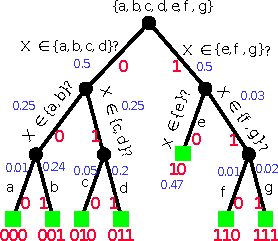
\includegraphics[width=0.9\linewidth]{figures/greedytree.pdf}
  \caption{Árvore obtida através do método guloso seguindo a estratégia \emph{top-down}.}\label{fig:greedytree}
  \end{marginfigure}

  A título de comparação, o algoritmo de Huffman produz o código apresentado na \Cref{fig:huffman}.
  Terá comprimento esperado $E l_{\text{huffman}} = 1.97$ e eficiência $H/E l_{\text{huffman}} = 0.9809$.

  Isto demonstra claramente que o código de Huffman é superior e que a estratégia gulosa
  não foi capaz de nos levar a um código ótimo.
  \begin{marginfigure}%
  \centering
  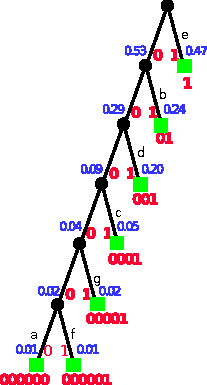
\includegraphics[width=0.7\linewidth]{figures/huffman.pdf}
  \caption{Árvore obtida pelo código de Huffman.}\label{fig:huffman}
  \end{marginfigure}
\end{example}


O algoritmo de Huffman pode ser sumarizado através dos seguintes passos:
\begin{enumerate}
\item Selecione os dois símbolos menos prováveis no alfabeto.
\item Ambos terão associados as palavras mais longas e se diferirão no último bit.
\item Combine estes dois símbolos em um símbolo auxiliar com probabilidade igual à soma das
        probabilidades dos dois símbolos. Adicione o símbolo auxiliar e remova os dois símbolos previamente selecionados.
        Repita os passos.
\end{enumerate}

O procedimento é similar para $D > 2$. Neste caso poderá ser necessário utilizar símbolos fictícios no alfabeto.

\begin{example}[\parencite{bilmes2013}]
Seja $\mathcal{X} = \{1,2,3,4,5\}$ com probabilidades $(1/4, 1/4, 1/5, 3/20, 3/20)$.
O procedimento e o código de Huffman obtido estão dispostos na \Cref{fig:ex-huffman01}.

       \begin{figure}[h!]
       \centering
       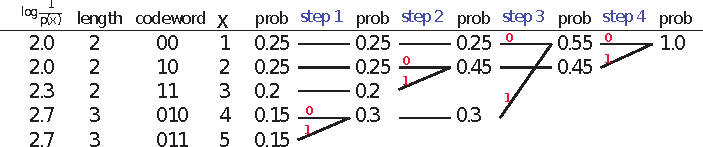
\includegraphics[width=0.95\textwidth]{figures/ex-huffman01.pdf}
       \caption{Código de Huffman exemplo.}\label{fig:ex-huffman01}
       \end{figure}

Para este código de Huffman teremos $E l = 2.3$ bits e $H=2.2855$ bits.
Note que, algumas palavras são maiores e outras menores que $l^\ast(x) = I(X) = \log 1/p(x)$.
O código de Huffman encontrado pode ser expresso, de maneira compacta, como: $((2,3),(1,(4,5)))$,
onde cada par de parênteses representada os símbolos combinados em cada passo do algoritmo.
\end{example}

O lema a seguir descreve atributos necessários para códigos de prefixo ótimos,
relacionando a frequência dos símbolos à estrutura de suas palavras. Ele
assegura que símbolos mais prováveis tenham comprimentos menores ou iguais e
que as duas palavras mais longas, ligadas aos símbolos menos frequentes,
possuam comprimentos iguais e difiram apenas no último bit. Essas propriedades,
intrínsecas a códigos ótimos, refletem a construção \emph{bottom-up} do algoritmo de
Huffman.


\begin{lemma}[Propriedades de Códigos Instantâneos Ótimos]\label{lem:propcodinstot}
Para toda distribuição, $\exists$ um código instantâneo ótimo (i.e., com comprimento esperado mínimo)
satisfazendo simultâneamente:
\begin{enumerate}
  \item\label{propcodinstot1} Se $p_j > p_k$ então $l_j \leq l_k$ (i.e., o símbolo mais provável não possui palavra com maior comprimento).
  \item\label{propcodinstot2} As duas maiores palavras possuem o mesmo comprimento.
  \item\label{propcodinstot3} As duas maiores palavras diferem apenas no último bit e correspondem aos dois símbolos menos prováveis.
\end{enumerate}
\end{lemma}

\begin{proof}
Vejamos primeiramente a propriedade \ref{propcodinstot1}.

Suponha que $C_m$ seja um código ótimo (então $L(C_m)$ é mínimo) e escolha $j,k$ de forma tal que $p_j > p_k$.
Precisamos mostrar que $\exists$ um código com $l_j \leq l_k$.
Considere o código $C_m'$ com a troca das palavras $j$ e $k$, ou seja,
\begin{equation}
  l_j' = l_k \quad \text{e} \quad l_k' = l_j ,
\end{equation}
o que só pode tornar o código maior, então $L(C_m') \geq L(C_m)$.

Realizando a troca, como $L(C_m)$ é mínimo, teremos
\begin{subequations}
  \begin{align}
    0 &\leq L(C_m') - L(C_m) = \sum_i p_i l_i' - \sum_i p_i l_i \\
      &= p_j l_j' + p_k l_k' - p_j l_j - p_k l_k = p_j l_k + p_k l_j - p_j l_j - p_k l_k \\
      &= p_j (l_k - l_j) - p_k (l_k - l_j) \\
      &= \underbrace{(p_j - p_k)}_{>0}  (l_k - l_j)
  \end{align}
\end{subequations}
Devemos ter então $(l_k - l_j) \geq 0$, ou seja, $l_k \geq l_j$ quando $p_j > p_k$, satisfazendo assim a propriedade \ref{propcodinstot1}.
Esta propriedade é verdadeira para todos códigos ótimos.

Vejamos agora a propriedade \ref{propcodinstot2}: as palavras mais longas possuem o mesmo comprimento.

Se as duas palavras maiores não possuem o mesmo comprimento, podemos apagar o último bit da palavra mais longa.
Desta forma manteremos a propriedade de prefixo, já que a palavra mais longa é a única com o seu dado comprimento e não
existe um prefixo dela que seja uma outra palavra (veja a \Cref{fig:lemmahuffman}).
 \begin{figure}[h!]
 \centering
 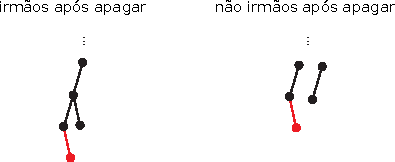
\includegraphics[width=0.5\textwidth]{figures/lemmahuffman.pdf}
 \caption{Apagando o último bit da palavra mais longa.}\label{fig:lemmahuffman}
 \end{figure}

Desta forma reduzimos o comprimento esperado. Concluímos que um código ótimo deve possuir as duas
palavras mais longas com o mesmo comprimento.

Analisaremos agora a propriedade \ref{propcodinstot3}: as duas palavras mais longas diferem apenas no último bit e correspondem aos símbolos menos prováveis.

Devido à propriedade 1 ($p_k < p_j \Rightarrow l_k \geq l_j$), se $p_k$ é a menor probabilidade, então ela deve
possuir associada uma palavra de comprimento que não seja menor do que qualquer outra $j$ com $p_j > p_k$.
De forma similar, se $p_k$ é a segunda menor probabilidade, a palavra associada deve possuir comprimento que não seja
menor do que qualquer outro símbolo mais provável.
As duas palavras mais longas possuem o mesmo comprimento (propriedade \ref{propcodinstot2}) e
correspondem aos dois símbolos menos prováveis.
Se as duas maiores palavras não são irmãs, podemos trocá-las. Isto é, se $p_1 \geq p_2 \geq \ldots \geq p_m$, então
fazemos a transposição ilustrada na \Cref{fig:lemmahuffman2}.

\begin{figure}[h!]
\centering
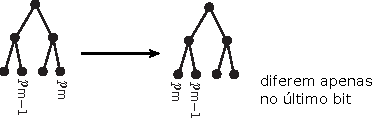
\includegraphics[width=0.5\textwidth]{figures/lemmahuffman2.pdf}
\caption{Transposição das duas palavras mais longas.}\label{fig:lemmahuffman2}
\end{figure}

Isto não altera o comprimento esperado $L = \sum_i p_i l_i$.
\end{proof}



O \Cref{lem:propcodinstot} nos fornece que, se $p_1 \geq p_2 \geq \ldots \geq p_m$, 
então existe um código ótimo com $l_1 \leq l_2 \leq \ldots l_{m-1} = l_m$
e no qual $C(x_{m-1})$ e $C(x_m)$ diferem apenas no último bit.

Vamos mostrar que Huffman é ótimo através da operação de criar um novo código no qual a otimização é mais simples.
Este processo é repetido até que a otimização seja trivial.

\begin{theorem}[Otimidade do Código de Huffman]\label{thm:optcodhuffman}
O procedimento de codificação de Huffman cria um código com comprimentos inteiros ótimo.
\end{theorem}
\begin{proof}
  
Assuma um código $C_m$ (não necessariamente ótimo) que satisfaz as propriedades anteriores.
$C_m$ terá as seguintes palavras de código $\{w_i\}_{i=1}^m$.
O procedimento de Huffman consiste em transformar $C_m$ em $C_{m-1}$, com palavras de código $\{w_i'\}_{i=1}^{m-1}$.
Para o código $C_m$ teremos as seguintes palavras, comprimento e probabilidades associados:
\begin{center}
  \begin{tabular}{ccc}
  $C_m$ & comprimento & prob. do símbolo \\ \hline
  $w_1$ & $l_1$ & $p_1$ \\
  $w_2$ & $l_2$ & $p_2$ \\
  $\vdots$ & $\vdots$ & $\vdots$ \\
  $w_{m-2}$ & $l_{m-2}$ & $p_{m-2}$ \\
  $w_{m-1}$ & $l_{m-1}$ & $p_{m-1}$ \\
  $w_{m}$ & $l_{m}$ & $p_{m}$ \\
  \end{tabular}
\end{center}

Para ir de $C_m$ para $C_{m-1}$, o procedimento de Huffman combina dos dois símbolos
de menor probabilidades em $C_m$, criando um símbolo auxiliar em $C_{m-1}$ com probabilidade
dada pela soma $p_{m-1}' = p_{m-1} + p_m$. A transformação de $C_m$ em $C_{m-1}$ é
esquematizada a seguir:
\begin{center}
  \begin{tabular}{cccccc}
  \scriptsize{prob. símb.} & $C_{m-1}$ & \scriptsize{comp.} $m-1$ & \scriptsize{rel. código} & \scriptsize{rel. comp.} & \scriptsize{prob. símb.} \\ \hline
  $p_1$   & $w_1'$        & $l_1'$        & $w_1 = w_1'$  & $l_1 = l_1'$  & $p_1$ \\
  $p_2$   & $w_2'$        & $l_2'$        & $w_2 = w_2'$  & $l_2 = l_2'$  & $p_2$ \\
  $\vdots$ & $\vdots$ & $\vdots$ & $\vdots$ & $\vdots$ & $\vdots$ \\
  $p_{m-2}$   & $w_{m-2}'$        & $l_{m-2}'$        & $w_{m-2} = w_{m-2}'$  & $l_{m-2} = l_{m-2}'$  & $p_{m-2}$ \\
  $p_{m-1} + p_m$   & $w_{m-1}'$        & $l_{m-1}'$        & $w_{m-1} = w_{m-1}' 0$  & $l_{m-1} = l_{m-1}'+1$  & $p_{m-1}$ \\
          &       &       & $w_{m} = w_{m-1}' 1$ & $l_m = l_{m-1}'+1$ & $p_m$
  \end{tabular}
\end{center}
onde $w_i$ e $l_i$ são as palavras e comprimento das palavras do código $C_m$ e $w_i'$ e $l_i'$ do código $C_{m-1}$.

As palavras e comprimentos em Huffman são definidos recursivamente. Huffman define uma relação entre palavras
(e consequentemente comprimentos) ao dar um passo de um código para outro mais simples.

Obtemos assim a seguinte relação entre o comprimento esperado de $C_m$ e o comprimento esperado de $C_{m-1}$:
\begin{subequations}
  \begin{align}
    L(C_m) &= \sum_i p_i l_i\\
           &= \sum_{i=1}^{m-2} p_i l_i' + p_{m-1} (l_{m-1}' + 1) + p_m (l_{m-1}' + 1) \\
           &= \sum_{i=1}^{m-2} p_i l_i' + (p_{m-1} + p_m) l_{m-1}' + p_{m-1} + p_m \\
           &= \sum_{i=1}^{m-1} p_i' l_i'+ p_{m-1} + p_m \\
           &= L(C_{m-1}) + p_{m-1} + p_m
  \end{align}
\end{subequations} 
onde o termo $p_{m-1} + p_m$ é constante, não envolve comprimentos de palavras e, consequentemente,
não tem nenhuma implicância no processo de otimização.

Desta forma, reduzimos o número de variáveis que iremos otimizar de $m$ para $m-1$.
O procedimento de Huffman implica em 
\begin{subequations}
  \begin{align}
    \min_{l_{1:m}} L(C_m) &= \text{const.} + \min_{l_{1:m-1}} L(C_{m-1}) \\
                          &= \text{const.} + \min_{l_{1:m-2}} L(C_{m-2}) \\
                          & \;\; \vdots \nonumber \\
                          &= \text{const.} + \min_{l_{1:2}} L(C_{2})
  \end{align}
\end{subequations}
onde em cada passo são preservadas as propriedades.

Ao reduzir para o caso com dois comprimentos ($C_2$), teremos a solução óbvia, um bit para cada símbolo, e assim 
podemos refazer o caminho de volta e construir o código.
Em cada passo garantimos que estaremos obtendo a solução ótima, e assim o código criado pelo algoritmo de Huffman
será ótimo.
\end{proof}





\section{Codificação Shannon-Fano-Elias}

A codificação Shannon-Fano-Elias é uma abordagem prática para representar
símbolos com base em suas probabilidades cumulativas. Ela atribui códigos
prefixo aproximando os comprimentos ideais por meio de uma representação
binária truncada da função de distribuição cumulativa. Historicamente,
Shannon-Fano-Elias é um marco na evolução da codificação, sendo ela
predecessora da codificação aritmética, que também usa probabilidades
cumulativas. 

Vejamos algumas definições que serão utilizadas na codificação Shannon-Fano-Elias.
\begin{definition}[Distribuição Cumulativa]
Seja $\mathcal{X} = \{x_1, x_2, \ldots, x_m\}$ um conjunto finito de símbolos 
com uma distribuição $p$, onde $p(x_i) \geq 0$ e $\sum_{i=1}^m p(x_i) = 1$.
A função de distribuição cumulativa, denotada por $F(x)$, é definida como:
\begin{equation}
F(x) = \sum_{a \leq x} p(a),
\end{equation}
em que a soma é tomada sobre todos os símbolos $a \in \mathcal{X}$ 
tais que $a \leq x$, considerando a ordenação de $\mathcal{X}$: 
$x_1 < x_2 < \cdots < x_m$. Assim, $F(x)$ representa a probabilidade acumulada
de todos os símbolos até $x$, inclusive, e satisfaz as propriedades: $0 \leq F(x) \leq 1$,
$F(x_i) \leq F(x_j)$ se $x_i < x_j$ (monotonicidade), e $F(x_m) = 1$. 
\end{definition}


\begin{definition}[\(\overline{F}\)-Distribuição Cumulativa Modificada]
Seja $\mathcal{X} = \{x_1, x_2, \ldots, x_m\}$ um conjunto finito de símbolos
com uma distribuição $p$, e seja $F(x) = \sum_{a \leq x} p(a)$ a função de
distribuição cumulativa associada, considerando uma ordenação fixa $x_1 < x_2 <
\cdots < x_m$. A função $\overline{F}(x)$, chamada de distribuição cumulativa
modificada, é definida como:
\begin{subequations}
\begin{align}
\overline{F}(x) &\triangleq \sum_{a < x} p(a) + \frac{1}{2} p(x), \\
&= F(x) - \frac{1}{2} p(x),
\end{align}
\end{subequations}
em que $\sum_{a < x} p(a)$ é a soma das probabilidades dos símbolos
estritamente menores que $x$, e $\frac{1}{2} p(x)$ adiciona metade da
probabilidade do símbolo $x$. Assim, $\overline{F}(x)$ representa um ponto
intermediário no intervalo de probabilidade associado a $x$ na distribuição
acumulada.
\end{definition}

$\overline{F}(x)$ é o ponto entre $F(x-1)$ e $F(x)$, então, como $p(x)>0$, temos
\begin{equation}
  F(x-1) < \overline{F}(x) < F(x)
\end{equation}

Como $p(x)>0$, $a \neq b \Rightarrow F(a) \neq F(b) \Leftrightarrow
\overline{F}(a) \neq \overline{F}(b)$.  Podemos utilizar $\overline{F}(a)$ como
um código não singular para $a$ (podemos utilizar a expansão binária após a
vírgula, como visto anteriormente na prova de Kraft para um infinito contável
de comprimentos).  Teremos um código unicamente decodificável, porém poderemos
ter palavras de tamanho infinito.  A solução será truncar $\overline{F}(x)$
para ficar com $l(x)$ bits. A notação para tanto será $\lfloor \overline{F}(x) \rfloor_{l(x)}$.

\begin{example}[Truncamento com $l$ bits]\label{ex:Fbarratruncado}
Seja $l=4$ e $\overline{F}(x) = 0.011011001000\ldots$, então
\begin{equation}
    \lfloor \overline{F}(x) \rfloor_{l(x)} = 0.0110 .
\end{equation}
    \centering{
    \begin{tabular}{ccccc}
	& 0.0110 & 1100 & 1000 & \\
    $-$ & 0.0110 & 0000 & 0000 & código $\lfloor \overline{F}(x) \rfloor_4$ \\
    \hline
    $=$ & 0.0000 & 1100 & 1000 & \\
    $<$ & 0.0001 & 0000 & 0000 & $= 1/2^{l(x)}$
    \end{tabular}
    }
\end{example}

Precisamos agora determinar qual seria $l(x)$ mínimo para que a decodificação unívoca seja preservada.
Sabemos que
\begin{equation}
 \overline{F}(x) - \lfloor \overline{F}(x) \rfloor_{l(x)} < \frac{1}{2^{l(x)}} ,
\end{equation}
conforme ilustrado no \Cref{ex:Fbarratruncado}.
Se considerarmos $l(x) = \lceil \log 1/p(x) \rceil + 1$, então teremos
\begin{subequations}
\begin{align}
\frac{1}{2^{l(x)}} &= \frac{1}{2} 2^{- \lceil \log 1/p(x) \rceil} \leq \frac{1}{2} 2^{-\log 1/p(x)} = \frac{p(x)}{2} \\
                &= \overline{F}(x) - F(x-1)
\end{align}
\end{subequations}
Combinando com o limite anterior, teremos
\begin{equation}
 \overline{F}(x) - \lfloor \overline{F}(x) \rfloor_{l(x)} < \frac{1}{2^{l(x)}} < \overline{F}(x) - F(x-1) ,
\end{equation}
e poderemos concluir que
\begin{equation}
 \lfloor \overline{F}(x) \rfloor_{l(x)} > F(x-1) .
\end{equation}
Por fim, temos
\begin{equation}
 F(x-1) < \lfloor \overline{F}(x) \rfloor_{l(x)} \leq \overline{F}(x) < F(x) .
\end{equation}

Concluímos que $l(x) = \lceil \log 1/p(x) \rceil + 1$ bits serão suficientes para descrever $x$ de forma não ambígua
segundo a representação $\lfloor \overline{F}(x) \rfloor_{l(x)}$, uma vez
que para cada $x$ teremos $\lfloor \overline{F}(x) \rfloor_{l(x)}$ em intervalos distintos, conforme a desigualdade anterior.

Precisamos agora verificar que a representação binária do $\lfloor \overline{F}(x) \rfloor_{l(x)}$ nos fornecerá
um código de prefixo. Para tanto, considere a palavra $z_1 z_2 \ldots z_l$ que corresponde ao intervalo semiaberto:
\begin{equation}
  [ \overbrace{0.z_1 z_2 \ldots z_l}^{\lfloor \overline{F}(x) \rfloor_{l(x)}} , \quad \overbrace{0.z_1 z_2 \ldots z_l}^{\lfloor \overline{F}(x) \rfloor_{l(x)}} + 1/2^l  ) =
  \left[ 0.z_1 z_2 \ldots z_l , \quad 0.z_1 z_2 \ldots z_l + 0.00\ldots 1  \right) .
\end{equation}
que possui comprimento $1/2^l$ (este intervalo contém todos os números binários que se iniciam com $0.z_1 z_2 \ldots z_l$).

A desigualdade $F(x-1) < \lfloor \overline{F}(x) \rfloor_{l(x)} \leq \overline{F}(x) < F(x)$ e o intervalo de comprimento $1/2^l$ são representados na
\Cref{fig:intervalshannonfanoelias}
\begin{marginfigure}%
  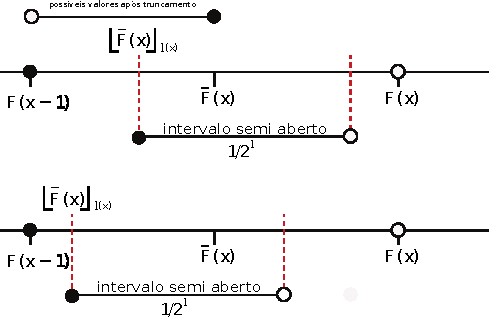
\includegraphics[width=\linewidth]{figures/intervalshannonfanoelias.pdf}
  \caption{Intervalo de comprimento $1/2^l$ representando $\lfloor \overline{F}(x) \rfloor_{l(x)}$ como uma forma não ambígua para codificação.}\label{fig:intervalshannonfanoelias}
\end{marginfigure}
Então $\lfloor \overline{F}(x) \rfloor_{l(x)} \in (F(x-1), \overline{F}(x)]$.
Como $2^{-l(x)} \leq p(x)/2 = \overline{F}(x) - F(x-1)$  e também $F(x-1) < \lfloor \overline{F}(x) \rfloor_{l(x)} \leq \overline{F}(x) < F(x)$, então
teremos que os intervalos abertos são disjuntos, mesmo se $\lfloor \overline{F}(x) \rfloor_{l(x)} = \overline{F}(x)$.
A forma de codificação proposta, usando a representação binária de $\lfloor \overline{F}(x) \rfloor_{l(x)}$, 
nos leva a um código de prefixo (não existirão duas palavras associadas a um mesmo intervalo e os intervalos associados a cada um são disjuntos).
Como é suficiente ter $l(x) = \lceil \log 1/p(x) \rceil + 1$, podemos calcular o limite para o comprimento esperado.
Assim,
\begin{equation}
 L = \sum_{x} p(x) l(x) = \sum_{x} p(x) (\lceil \log 1 / p(x) \rceil + 1) \leq H(X) + 2
\end{equation}


\begin{example}[Distribuição d-ádica]
Considere a seguinte distribuição d-ádica. Os passos para 
encontrar o código de Shannon-Fano-Elias são explicitados 
abaixo.

\begin{center}
  \begin{tabular}{lllllll}
  $x$ & $p(x)$ & $F(x)$ & $\overline{F}(x)$       & $\overline{F}(x)$ (binário) & $l(x)$ & palavra código \\ \hline
  1   & 0.25   & 0.25   & 0.125           & 0.001                 & 3     & 001   \\
  2   & 0.5    & 0.75   & 0.5             & 0.10                  & 2     & 10    \\
  3   & 0.125  & 0.875  & 0.8125          & 0.1101                & 4     & 1101  \\
  4   & 0.125  & 1.0    & 0.9375          & 0.1111                & 4     & 1111
  \end{tabular}
\end{center}

Para o código encontrado teremos $El = 2.75$ bits enquanto $H=1.75$ bits. 
Comparativamente, para o caso de Huffman teremos a árvore $(((3,4),1),2)$, 
e assim $El_{\text{huffman}} = 0.25 \time 1 + 0.25 \times 2 + 0.125 \times 3 + 0.125 \times 3 = 1.75$.
\end{example}


\begin{example}[Dízima periódica]
Utilizaremos a seguinte notação para dízima periódica: $0.\overline{01} = 0.010101010101\ldots$.
Para uma dada distribuição $p$, abaixo apresentamos os passos para
encontrar o código de Shannon-Fano-Elias:

\begin{center}
  \begin{tabular}{lllllll}
  $x$ & $p(x)$ & $F(x)$ & $\overline{F}(x)$    & $\overline{F}(x)$ (binário) & $l(x)$ & palavra código \\ \hline
  1   & 0.25   & 0.25   & 0.125           & $0.001$                 & 3     & 001   \\
  2   & 0.25   & 0.5    & 0.375           & $0.011$                 & 3     & 011   \\
  3   & 0.2    & 0.7    & 0.6             & $0.1\overline{0011}$         & 4     & 1001  \\
  4   & 0.15   & 0.85   & 0.775           & $0.110\overline{0011}$       & 4     & 1100  \\
  5   & 0.15   & 1      & 0.925           & $0.111\overline{0110}$          & 4     & 1110
  \end{tabular}
\end{center}
Para o código de Shannon-Fano-Elias encontrado, teremos $H=2.285$ bits, $El = 3.5$ bits, 
enquanto $El_{\text{huffman}} = 2.3$ bits, sendo a árvore de Huffman $((1,(4,5)),(3,2))$.
\end{example}
















\section{O Jogo de Shannon}

A compreensão da entropia como medida da incerteza em uma fonte de informação é
fundamental para o desenvolvimento de códigos eficientes. Em seu artigo de
1951~\parencite{Shannon1951}, \textit{``Prediction and Entropy of Printed English''}, Claude Shannon
explorou essa ideia por meio de um experimento simples,
conhecido como o Jogo de Shannon. Neste jogo, participantes tentam adivinhar a
próxima letra em uma sequência de texto em inglês, como completar ``TH'' em
``THE'' ou ``THEN'', utilizando o contexto das letras anteriores. Shannon
observou que, em média, os participantes precisavam de poucas tentativas para
acertar, sugerindo que a previsibilidade do idioma reduz significativamente a
quantidade de informação por letra.

Para quantificar isso, Shannon modelou o texto como um processo estocástico e
estimou a entropia condicional --- a incerteza média de uma letra dado o
contexto anterior. Usando amostras de até 100 letras e aproximações estatísticas
(de monogramas, bigramas e trigramas), ele concluiu que a entropia do inglês impresso
está entre 0,6 e 1,3 bits por letra, muito abaixo dos 4,76 bits de um alfabeto
de 27 símbolos (26 letras mais espaço) com distribuição uniforme. Esse
resultado implica uma redundância de cerca de 75\%, evidenciando que a
estrutura linguística permite compressão eficiente.

O Jogo de Shannon destaca a
dependência entre símbolos em uma sequência. Por exemplo, após ``QU'', a
próxima letra é quase certamente uma vogal, reduzindo a incerteza. Essa visão
sequencial motiva alguns métodos, como a codificação aritmética, que
comprime uma mensagem inteira em um único número, aproveitando a entropia de
toda a sequência.









\section{Codificação Aritmética}

A codificação aritmética supera as limitações dos códigos baseados em símbolos
individuais, sendo considerada como um código de fluxo, ou seja, codifica uma
sequência inteira em um único número real/binário. Ao mapear a mensagem em um
intervalo de probabilidade que se estreita iterativamente com base nas
probabilidades cumulativas dos símbolos, a codificação aritmética alcança taxas
de compressão que se aproximam da entropia da fonte, mesmo em distribuições
complexas com dependências entre símbolos. O algoritmo básico da codificação
aritmética foi desenvolvido independentemente por Jorma Rissanen e Richard C.
Pasco, na década de 1970. A ideia reflete uma evolução natural das propostas de
Shannon, oferecendo uma solução elegante para fontes onde a redundância
sequencial desempenha um papel importante.

A codificação aritmética opera dividindo subsequentemente um intervalo inicial
de probabilidade, $[0, 1)$, com base nas probabilidades dos
símbolos de uma sequência. Para cada novo símbolo, o intervalo atual é
particionado proporcionalmente às probabilidades cumulativas dos símbolos
possíveis, e o subintervalo correspondente ao símbolo observado é selecionado.
À medida que a sequência avança, esse processo gera intervalos cada vez
menores, cuja largura reflete a probabilidade conjunta da sequência inteira.
Para transmitir a mensagem, escolhe-se um número binário que caiba dentro do
intervalo final --- tipicamente, uma sequência binária cuja representação
decimal esteja contida nesse intervalo reduzido. Esse número único codifica
toda a sequência.

Suponha que o alfabeto da fonte seja $\mathcal{X} = \{a_1, a_2, \ldots, a_I\}$.
À medida que a fonte produz uma sequência de símbolos $x_1, x_2, \ldots, x_n, \ldots$,
o intervalo real $[0, 1)$ é subsequentemente subdividido de acordo com
as probabilidades dos símbolos em cada instante. A \Cref{fig:acoding_invervals}
apresenta a subdivisão do intervalo para os dois primeiros símbolos da sequência.

\begin{figure}%
  \centering
  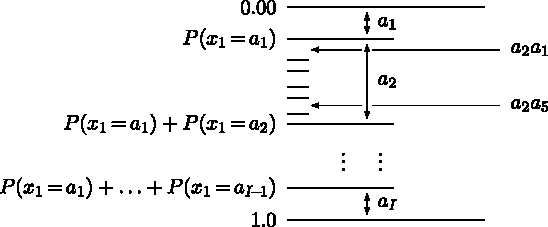
\includegraphics[width=0.75\linewidth]{figures/acoding_invervals.pdf}
  \caption{Definição dos intervalos probabilísticos para uma sequência de símbolos produzida pela fonte.}\label{fig:acoding_invervals}
\end{figure}

Paralelamente, o codificador deve ir subdividindo o intervalo $[0, 1)$,
sempre ao meio em cada passo, para determinar uma sequência binária
correspondente a um intervalo que esteja dentro do intervalo selecionado
pela sequência de símbolos produzida pela fonte.
A \Cref{fig:acoding_binaryinvervals} apresenta a subdivisão binária dos intervalos.

\begin{marginfigure}%
  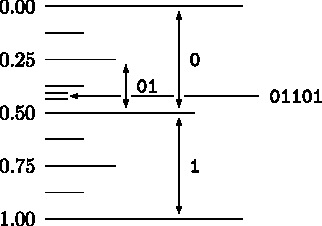
\includegraphics[width=\linewidth]{figures/acoding_binaryinvervals.pdf}
  \caption{Definição dos intervalos probabilísticos para uma sequência binária na saída do codificador.}\label{fig:acoding_binaryinvervals}
\end{marginfigure}




\begin{example}[\parencite{mackay2003}]
Suponha $x \in \{a,b,\square\}$, onde $\square$ é o símbolo de término.
Vamos considerar a codificação da \textit{string} $bbba\square$.
A seguir, apresentamos as probabilidades do próximo símbolo, dado o passado:

\begin{center}
  \begin{tabular}{cccc}
  -  & $p(a) = 0.425$ & $p(b) = 0.425$ & $p(\square) = 0.15$ \\
  $b$  & $p(a|b) = 0.28$ & $p(b|b) = 0.57$ & $p(\square | b) = 0.15$ \\
  $bb$ & $p(a|bb) = 0.21$ & $p(b|bb) = 0.64$ & $p(\square | bb) = 0.15$ \\
  $bbb$ & $p(a|bbb) = 0.17$ & $p(b|bbb) = 0.68$ & $p(\square | bbb) = 0.15$ \\
  $bbba$ & $p(a|bbba) = 0.28$ & $p(b|bbba) = 0.57$ & $p(\square | bbba) = 0.15$
  \end{tabular}
\end{center}

Temos subintervalos semiabertos em $[0,1)$.
Os intervalos $[l,u)$ são dados pela probabilidade condicional $p(x_i | x_1, x_2, \ldots, x_{i-1})$.
Temos a representação de um prefixo $b_1 b_2 \ldots b_k$ por um intervalo da forma
$[0.b_1 b_2 \ldots b_k, 0.b_1 b_2 \ldots b_k + 2^{-k})$ para $b_i \in \{0,1\}$.

\begin{marginfigure}%
  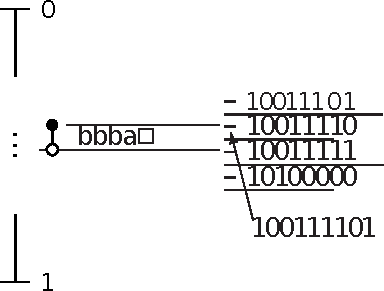
\includegraphics[width=\linewidth]{figures/bbba.pdf}
  \caption{Intervalo final para a sequências de símbolos da fonte e para a sequência binária na saída do codificador.}\label{fig:bbba}
\end{marginfigure}

A \Cref{fig:bbba} ilustra os intervalos que teremos ao final da sequência $bbba\square$
a ser codificada. Observe que a sequência binária $100111101$ correspondente a um
intervalo completamente dentro do intervalo associado à sequência $bbba\square$,
codificando assim a sequência da fonte.

A \Cref{fig:bbbaall} apresenta todo o processo de subdivisão dos intervalos.
 
\begin{figure}[h!]
\centering
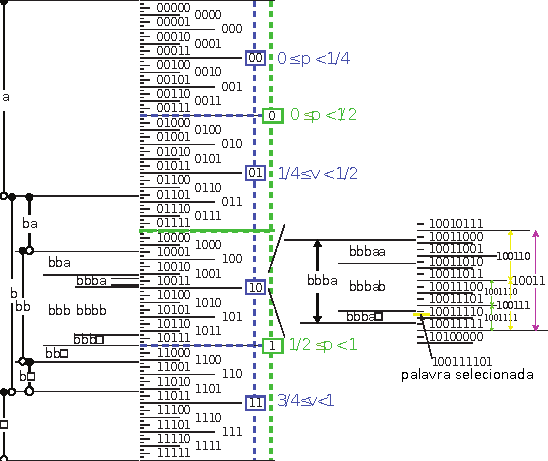
\includegraphics[width=\textwidth]{figures/bbbaall.pdf}
\caption{Todo o processo de subdivisão dos intervalos para a sequências de símbolos da fonte e para a sequência binária na saída do codificador \parencite{mackay2003}.}
\label{fig:bbbaall}
\end{figure}

\end{example}


